\section{Functional Requirements}
    This section is split into 3 parts, one for each application. In each of them there is a scenario describing a realistic situation that may occur in the world and how the actors interact with the software. Every scenario is then generalised in an use case diagram, several use cases,  sequence and activity diagrams from the UML framework.
    \subsection{Data4Help}
        Consider the following scenario:
        
        RestAssured is an insurance company that wants to offer a personalised service to its customers. In order to do so, it registers to \emph{Data4Help} as a Third-party through the Enterprise Android application, providing the needed data. Luigi is a new customer of RestAssured. The company has a special offer dedicated to the clients that accept to be tracked through \emph{Data4Help}, so he downloads the application on his device and registers to the service as an Individual, also associating his smart-watch. RestAssured then looks for him in the application inserting his fiscal code and sends him a request for the access to his data, including a subscription request, with updates wanted every week. Luigi accepts the request, so \emph{Data4Help} starts sending his data to RestAssured.
        
        After a couple of months, however, Luigi no longer wishes to benefit from RestAssured's special offer, because he is concerned about his privacy and finds out through \emph{Data4Help} that he is giving a lot of data to RestAssured. Therefore, he accesses the subscription page on \emph{Data4Help} and cancels the company's subscription. RestAssured receives the email that notifies Luigi's refusal of further provision of data and cancels his offer.
        
        Having a large client base, RestAssured decides to perform a statistical study on the health status of his customers. The company wants to start from Milan, so it performs an aggregated research on \emph{Data4Help}, setting the location to Milan and the time frame to the last month. Since the research produced more than 1000 results, \emph{Data4Help} sends the result back to the company, making the data anonymous.
        
            \begin{figure}[H]
                \centering
                \makebox[\textwidth][c]{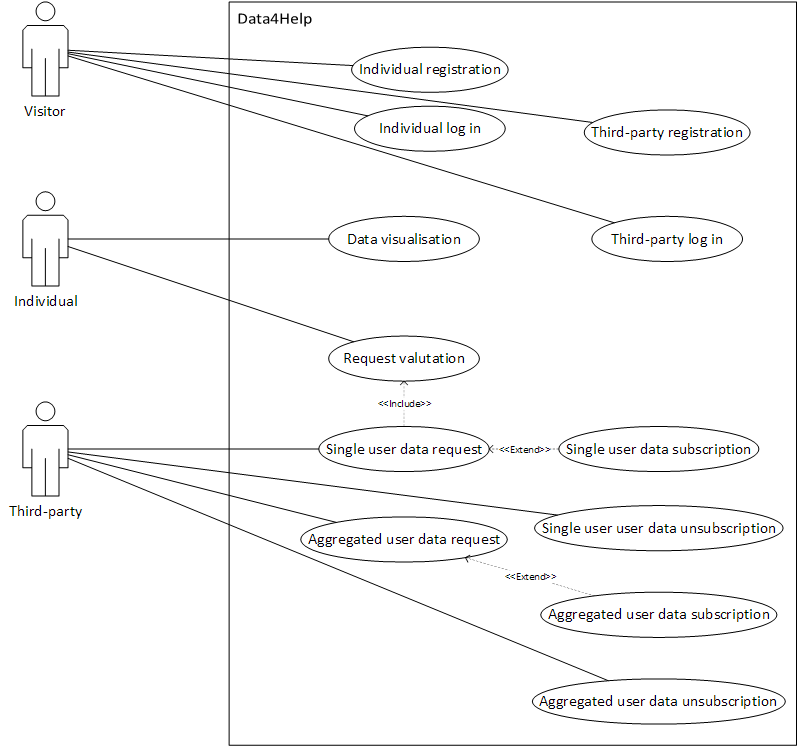
\includegraphics[scale=0.60]{pictures/D4H_UseCaseDiagram.png}}
                \caption{Use case diagram relative to \emph{Data4Help}.}
                \label{fig:D4H-Use-case-diagram}
            \end{figure}
        
        \subsubsection{Individual registration and log in}
            Every user who wants to use \emph{D4H} should be registered to the application System. After registration the user has to sign in, in order to collect data. \\

            \begin{table}[H]
            
            	\centering
                
                \begin{tabular}{|p{3cm}|p{8.2cm}|}
                    \hline
                    \textbf{Actors} & \begin{itemize}
                                          \item Visitor
                                          \item Individual
                                      \end{itemize} \\
                     \hline
                    \textbf{Entry Condition} & The user who wants to register must have a smart-watch or fitness-band\\
                     \hline
                    \textbf{Events Flow} & \begin{enumerate}
                                                \item The Visitor accesses the application log in page.
                                                \item The Visitor clicks on the ``\emph{Sign up now}" button and then fills in all the mandatory information (name, surname, fiscal code, password and email) in order to create an Individual account.
                                                \item The D4H System registers the user and sends back a confirmation email.
                                                \item The Visitor has to associate his smart-watch or fitness-band to the account.
                                                \item The Visitor becomes an Individual, inserting its email and password in the log in page.
                                            \end{enumerate}\\
                     \hline
                    \textbf{Exit Condition} & Now the user has his personal account.\\
                     \hline
                    \textbf{Exception} & The Registered user is not able to sign in the System because the ID (fiscal code for Individual) or password are wrong or he did not confirmed his email. In these situations, the system will show the user an error message.\\
                     \hline
                \end{tabular}  
            \end{table}
            
            \begin{figure}[H]
                \centering
                \makebox[\textwidth][c]{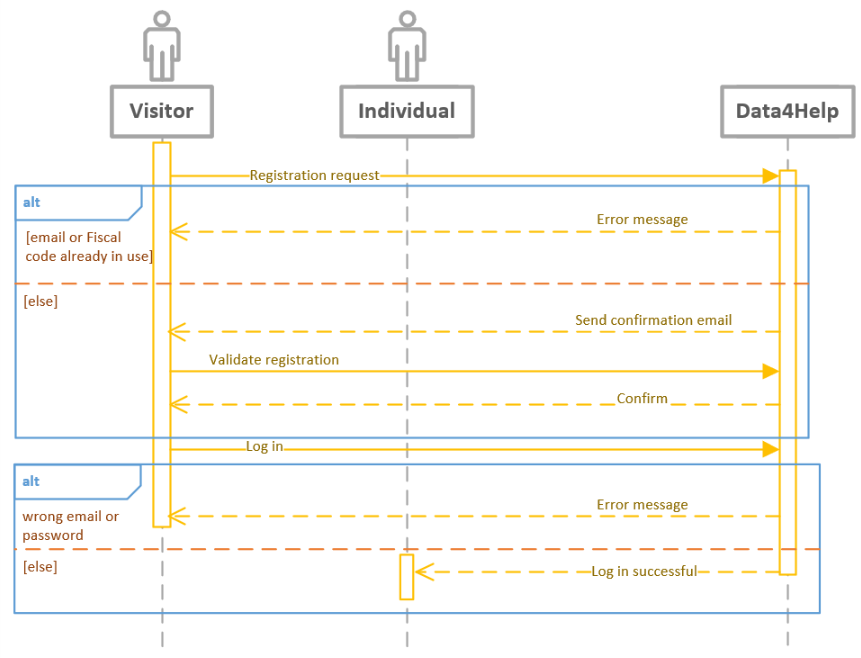
\includegraphics[scale=0.70]{pictures/IndividualRegistrationSequenceDiagram.png}}
                \caption{Sequence diagram representing the registration/log in phase of an Individual.}
                \label{fig:seq-diagram1}
            \end{figure}
        
        \subsubsection{Third-party registration and log in}
            In order to have access to the functionalities of the application, Visitors have to register to the service as Third-parties. After that, they will be able to log into the application using their email and password and to perform their researches.
            
            \begin{table}[H]
            	\centering
                \begin{tabular}{|p{3cm}|p{8.2cm}|}
                    \hline
                    \textbf{Actors} &  \begin{itemize}
                        \item Visitor
                        \item Third-party
                    \end{itemize} \\
                     \hline
                    \textbf{Entry Condition} & There is no entry condition. \\
                     \hline
                    \textbf{Events Flow} & \begin{enumerate}
                        \item The Visitor accesses the registration page of the Enterprise application.
                        \item The Visitor clicks on the ``\emph{Sign up now}" button and then fills in all the necessary information useful to be recognised as Third-party (company name, VAT code, email and password).
                        \item \emph{Data4Help} creates a new account and sends a confirmation email to the just registered Third-party.
                        \item The newly registered Third-party can now log into the application using the email and password previously provided, so to have access to the available features.
                    \end{enumerate} \\
                     \hline
                    \textbf{Exit Condition} & The Third-party is registered and able to log into \emph{Data4Help}. \\
                     \hline
                    \textbf{Exception} & The Visitor is not able to register because the email or the VAT code                      are already in use. \newline
                                         A registered Third-Party is not able to log in because the email or password inserted are wrong or the email has not been confirmed. \newline
                                         These exceptions will be handled by the system sending an error message. \\
                     \hline
                \end{tabular}  
            \end{table}
            
            \begin{figure}[H]
                \centering
                \makebox[\textwidth][c]{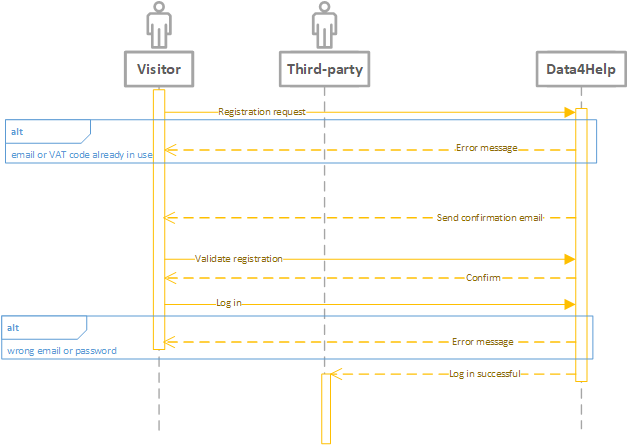
\includegraphics[scale=0.73]{pictures/RegistrationSequenceDiagram.png}}
                \caption{Sequence diagram representing the registration/log in phase of a Third-party.}
                \label{fig:seq-diagram2}
            \end{figure}
            
            
        \subsubsection{Single user data request and subscription}
  
            Third-parties can perform a request to Data4Help for a specific user by specifying his/her fiscal code. Data4Help forwards it to the Individual that can accept or refuse it. Then, in case of positive answer, Data4Help sends the user's health data to the applicant. If it is not, it sends a notification to the Third-party informing it about the refuse.

            \begin{table}[H]
            	\centering
                
                \begin{tabular}{|p{3cm}|p{8.2cm}|}
                    \hline
                    \textbf{Actors} &  \begin{itemize}
                                            \item Third-party
                                            \item Individual
                                        \end{itemize}\\
                     \hline
                    \textbf{Entry Condition} & Third-party has to be registered to Data4Help and logged in.\\
                     \hline
                    \textbf{Events Flow} & \begin{enumerate}
                                                \item The Third-Party selects ``\emph{Individual Request}" and it inserts the Fiscal Code of the desired person and, if it wants to subscribe, granularity and frequency of update.
                                                \item The System receives the request.
                                                \item The System looks for the user connected to the Fiscal Code requested and forwards him/her the request.
                                                \item The Individual receives the request with the name of the company that is requesting his/her data.
                                                 \item The Individual can accept or refuse the request. By accepting it, he/she allows the System to send all his/her health data to the applicant.
                                                 \item The system send notification to the Third-party.
                                            \end{enumerate}\\
                     \hline
                    \textbf{Exit Condition} & The Third-party has the user's collected data and receives updates of them periodically, if it has a subscription. \\
                     \hline
                    \textbf{Exception} & The Fiscal Code requested doesn't match with any registered user. In this case, the system notifies it with a pop-up in the Third-party application.\\
                     \hline
                \end{tabular}  
            \end{table} 
            
            \begin{figure}[H]
                \centering
                \makebox[\textwidth][c]{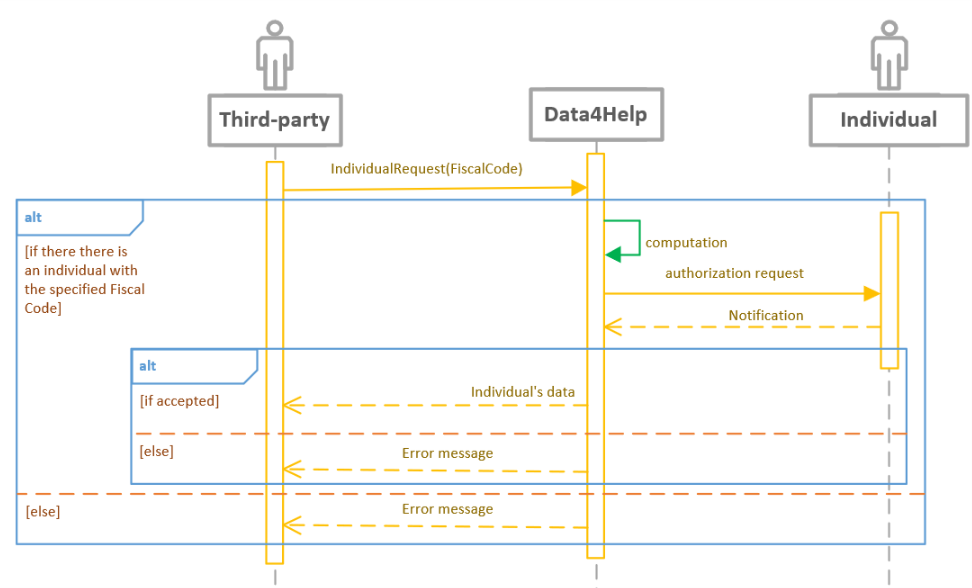
\includegraphics[scale=0.73]{pictures/IndividualRequestSequenceDiagram.png}}
                \caption{Sequence diagram representing the third-party Individual request.}
                \label{fig:IndividualRequest}
            \end{figure}
            
        
            
        \subsubsection{Aggregated user data request and subscription}
            Third-parties can perform group queries, asking for data coming from several Individuals that are within certain parameters specified by them (geographical areas, age, genre, time of the day). These requests are evaluated directly by D4H, that sends back the requested data only if the number of Individuals involved in the research is greater than 1000. If this is not the case, D4H sends an error message to the Third-party.

            \begin{table}[H]
            	\centering
                \begin{tabular}{|p{3cm}|p{8.2cm}|}
                    \hline
                    \textbf{Actors} &  \begin{itemize}
                        \item Third-party
                    \end{itemize} \\
                     \hline
                    \textbf{Entry Condition} & The Third-party is logged in. \\
                     \hline
                    \textbf{Events Flow} & \begin{enumerate}
                        \item The Third-party clicks on the ``\emph{Group request}" button.
                        \item The Third-party inserts the parameters of interest  and, if it wants to subscribe, granularity and frequency of update.
                        \item The Third-party decides whether it wants to subscribe to this particular research by checking the specific box or not, then clicks on the ``\emph{Search}" button to have D4H perform the multiple search.
                        \item \emph{Data4Help} does the research and evaluates the results.
                        \item D4H sends back the result to the Third-party.
                    \end{enumerate} \\
                     \hline
                    \textbf{Exit Condition} & The Third-party receives the requested information. \\
                     \hline
                    \textbf{Exception} & The number of Individuals involved in the multiple search is lower than 1000, therefore D4H sends an error message back to the Third-party. \\
                     \hline
                \end{tabular}  
            \end{table}
            
            \begin{figure}[H]
                \centering
                \makebox[\textwidth][c]{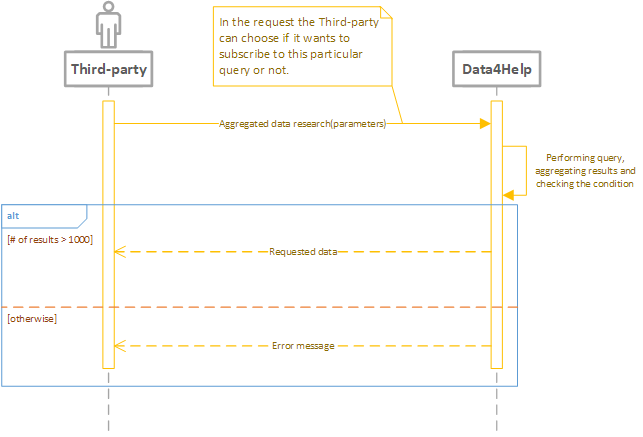
\includegraphics[scale=0.73]{pictures/Sequence2.png}}
                \caption{Sequence diagram representing the group requests performed by the Third-party.}
                \label{fig:Group-request-sequence-diagram}
            \end{figure}
            
        \subsubsection{Collected data during Subscription}    
            After a successful subscription request, the system sends updates to the Third-party aggregating the data with the specified granularity and frequency.
        
            \begin{table}[H]
            	\centering
                
                \begin{tabular}{|p{3cm}|p{8.2cm}|}
                    \hline
                    \textbf{Actors} &  \begin{itemize}
                                            \item Third-party
                                        \end{itemize}\\
                     \hline
                    \textbf{Entry Condition} & Third-party is logged in and has previously subscribed to the Individual's data.\\
                     \hline
                    \textbf{Events Flow} & \begin{enumerate}
                        \item When data arrived, the system checks if the Third-party is subscribed to single or aggregated user data.
                        \item If it is subscribed to aggregated user data, D4H evaluates the results.
                        \begin{itemize}
                            \item If results are less than 1000, the system deletes the subscription and sends an error message to the Third-party.
                        \end{itemize}
                        \item The system sends updates to the Third-party aggregating the data with the specified granularity and frequency. \end{enumerate}\\
                     \hline
                    \textbf{Exit Condition} & Third-party receives updated data with specified granularity and frequency. \\
                     \hline
                    \textbf{Exception} & The system goes out from loop when
                    \emph{Single User data unsubscription} or \emph{Aggregated user data unsubscription} starts, depending on what kind of data the Third-party is subscribed to. \\
                     \hline
                \end{tabular}  
            \end{table} 
            
             \begin{figure}[H]
                \centering
                \makebox[\textwidth][c]{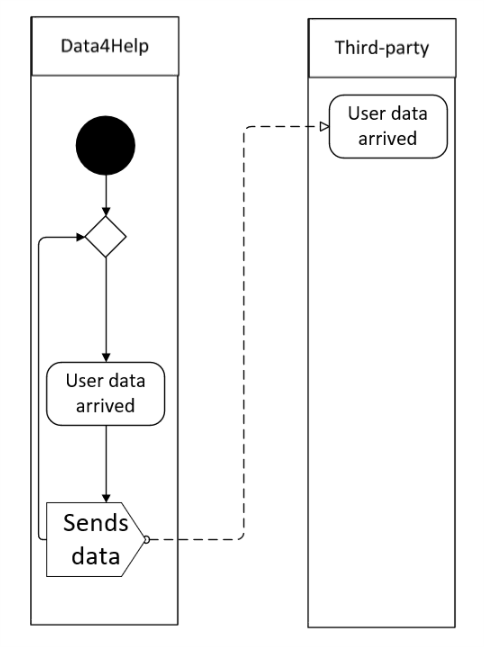
\includegraphics[scale=0.80]{pictures/SubscribedDataActivityDiagram.png}}
                \caption{Activity diagram represents data sending during subscription.}
                \label{fig:Sending-subscribed-data}
            \end{figure}
            
        \subsubsection{Single User data unsubscription}
            After a successful subscription request, both Third-parties and Individuals can make a request in order to cancel the subscription to the specified data.

            \begin{table}[H]
            	\centering
                
                \begin{tabular}{|p{3cm}|p{8.2cm}|}
                    \hline
                    \textbf{Actors} &  \begin{itemize}
                                            \item Third-party
                                            \item Individual
                                        \end{itemize}\\
                     \hline
                    \textbf{Entry Condition} & Third-party is logged in and has previously subscribed to the Individual's data.\\
                     \hline
                    \textbf{Events Flow} & \begin{enumerate}
                                                \item The Third-Party or Individual accesses to the subscription page and selects the subscription to be cancelled.
                                                \item The Third-party or the Individual presses ``\emph{Unsubscribe}" button.
                                                \item The system deletes the Third-party subscription and sends an email to both Third-party and Individual.
                                            \end{enumerate}\\
                     \hline
                    \textbf{Exit Condition} & The Third-party is not subscribed anymore, but it has access to the previously received data. \\
                     \hline
                    \textbf{Exception} & There are no exceptions. \\
                     \hline
                \end{tabular}  
            \end{table} 
            
            \begin{figure}[H]
                \centering
                \makebox[\textwidth][c]{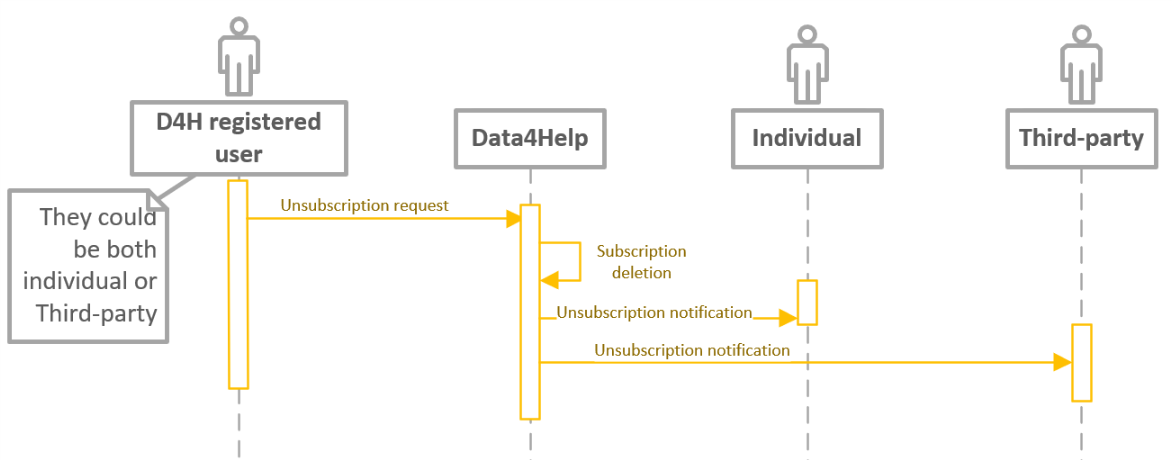
\includegraphics[scale=0.60]{pictures/IndividualRequestUnsubscriptionSequenceDiagram.png}}
                \caption{Sequence diagram representing the Unsubscription process for an individual data subscription.}
                \label{fig:Individual-request-unsubscription-process-sequence-diagram}
            \end{figure}    
            
        \subsubsection{Aggregated user data unsubscription}
        After a successful subscription to a group search, a Third-party can cancel it at any time if it does not wish to receive any further update. He will, however, still have access to the data collected until that point.
        
            \begin{table}[H]
            	\centering
                \begin{tabular}{|p{3cm}|p{8.2cm}|}
                    \hline
                    \textbf{Actors} &  \begin{itemize}
                        \item Third-party
                    \end{itemize} \\
                     \hline
                    \textbf{Entry Condition} & The Third-party is logged in and has previously subscribed to a group search. \\
                     \hline
                    \textbf{Events Flow} & \begin{enumerate}
                        \item The Third-Party accesses to the subscription page and selects the subscription to be cancelled.
                        \item The Third-party presses the ``\emph{Unsubscribe}" button.
                        \item The system deletes the Third-party subscription and sends an email to it for confirmation.
                    \end{enumerate} \\
                     \hline
                    \textbf{Exit Condition} & The Third-party is not subscribed anymore, but it has access to the previously received data. \\
                     \hline
                    \textbf{Exception} & There are no exceptions. \\
                     \hline
                \end{tabular}  
            \end{table}        
        
            \begin{figure}[H]
                \centering
                \makebox[\textwidth][c]{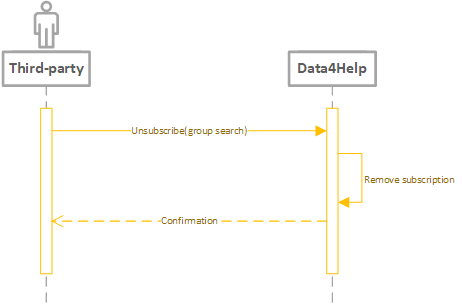
\includegraphics[scale=0.73]{pictures/Sequence3.png}}
                \caption{Sequence diagram representing the unsubscription from a group search by a Third-party.}
                \label{fig:Group-request-unsubscription-process-sequence-diagram}
            \end{figure}
        
        \subsubsection{Data Collection and Visualisation}
            
            Upon registration, Individuals allows the D4H system to collect their data and store them. To gather data, it's mandatory to have a device (smart-watch or fitness-band).
            
            \begin{table}[H]
            	\centering
                
                \begin{tabular}{|p{3cm}|p{8.2cm}|}
                    \hline
                    \textbf{Actors} & \begin{itemize}
                        \item Individual
                    \end{itemize} \\
                     \hline
                    \textbf{Entry Condition} & The user is correctly registered and logged into the D4H system. \\
                     \hline
                    \textbf{Events Flow} & \begin{enumerate}
                                                \item Smart-watch or fitness-band samples specific data.
                                                \item This device sends acquired data to D4H system.
                                                \item The system stores data and makes them visible to the owner Individual.
                                            \end{enumerate}\\
                     \hline
                    \textbf{Exit Condition} & The Individual has personal data stored in his D4H account.\\
                     \hline
                    \textbf{Exception} & If the associate device (smart-watch or fitness-band) does not work or does not send data anymore the exception will be handled by the system by sending an error message. \\
                     \hline
                \end{tabular}  
            \end{table} 
            
            \begin{figure}[H]
                \centering
                \makebox[\textwidth][c]{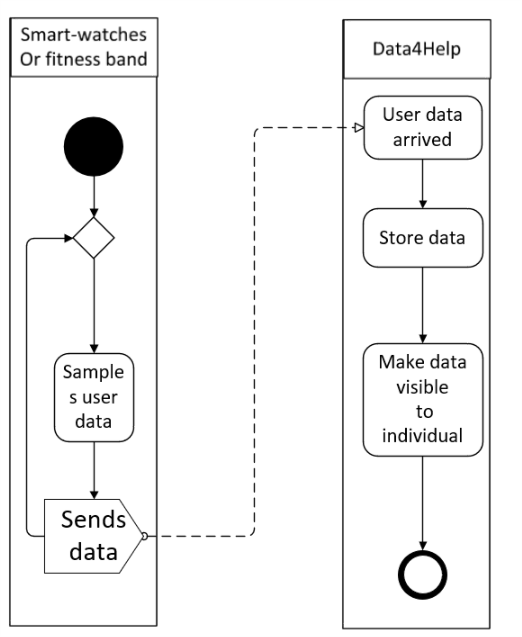
\includegraphics[scale=0.60]{pictures/DataStorageActivityDiagram.png}}
                \caption{Activity diagram representing data storage process.}
                \label{fig:Data-storage-activity-diagram}
            \end{figure}
            
        \subsubsection{Third-parties request history}
            Third-parties are able to see all of the requests that they have done and still have access the data of the ones that were approved at the time.
            
            \begin{table}[H]
            	\centering
                
                \begin{tabular}{|p{3cm}|p{8.2cm}|}
                    \hline
                    \textbf{Actors} & \begin{itemize}
                                            \item Third-party
                                        \end{itemize} \\
                     \hline
                    \textbf{Entry Condition} & The Third-party is logged in and has made at least a request. \\
                     \hline
                    \textbf{Events Flow} & \begin{enumerate}
                                                \item The Third-party clicks on the ``\emph{Request history}" tab.
                                                \item The Third-party selects the request of which it wishes to see the details.
                                                \item D4H shows the details (and the data, if the request was approved) to the Third-party.
                                            \end{enumerate} \\
                     \hline
                    \textbf{Exit Condition} & The Third-party is able to see the details of the                                  selected request it has previously made. \\
                     \hline
                    \textbf{Exception} & If the Third-party has not performed any request, an error                         message is sent to it. \\
                     \hline
                \end{tabular}  
            \end{table}
            
            \begin{figure}[H]
                \centering
                \makebox[\textwidth][c]{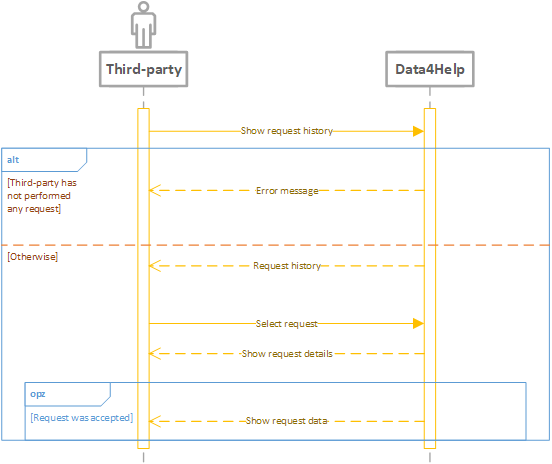
\includegraphics[scale=0.84]{pictures/modelD4H_ThirdPartyRequestHistory.png}}
                \caption{Sequence diagram representing the way a Third-party can access his request history.}
                \label{fig:D4H-Third-party-request-history}
            \end{figure}
            
            
    \subsection{AutomatedSOS}
        Consider the following scenario:
        
        Leo is a 67 years old man, already registered to \emph{Data4Help}. After the company has enabled \emph{AutomatedSOS} service, he is asked if he wants to subscribe to it for an additional price. He accepts and then \emph{TrackMe} sends him the instructions to follow in order to activate the service. Therefore, Leo opens \emph{AutomatedSOS}. After that, he clicks the button to subscribe. \emph{AutomatedSOS} evaluates and accepts the request (since Leo is 67).
        
        One day, Leo is taken ill suddenly and his hearth rate goes below 40 bpm. The fitness band measures this value, sends it to \emph{Data4Help} that forwards it to \emph{AutomatedSOS}. The software recognises the measurement as critical and promptly sends to the ambulance service Leo's data and location. Within 5 minutes, an ambulance arrives at Leo's house and brings him to the hospital.

        \begin{figure}[H]
            \centering
            \makebox[\textwidth][c]{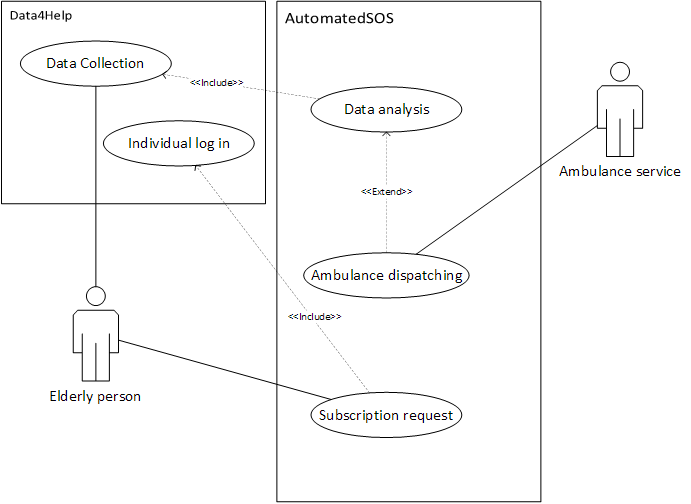
\includegraphics[scale=0.67]{pictures/ASOS_UseCaseDiagram.png}}
            \caption{Use case diagram relative to \emph{AutomatedSOS}. You can see the full use case diagram of D4H in the figure \ref{fig:D4H-Use-case-diagram}.}
            \label{fig:ASOS-Use-case-diagram}
        \end{figure}

        \subsubsection{Subscription Request}
            
            Every Individual (user registered to D4H) can ask for subscription to AutomatedSOS service, but only Elderly people will be allowed to use it.
            
            \begin{table}[H]
            	\centering
                
                \begin{tabular}{|p{3cm}|p{8.2cm}|}
                    \hline
                    \textbf{Actors} & \begin{itemize}
                        \item Individual
                    \end{itemize} \\
                     \hline
                    \textbf{Entry Condition} & The user has a D4H account and is logged in. \\
                     \hline
                    \textbf{Events Flow} & \begin{enumerate}
                                               \item The Individual presses on
                                               ``\emph{AutomatedSOS service}", in order to make a new subscription request, then clicks on the ``\emph{Subscribe}" button.
                                               \item The ASOS System checks if the petitioner is at least 65 years old.
                                               \item If verified, the user gets subscribed.
                                           \end{enumerate} \\
                     \hline
                    \textbf{Exit Condition} & The Individual is now subscribed to Automated SOS service.\\
                     \hline
                    \textbf{Exception} & If the petitioner is less then 65 years old, the system handles the exception, sending him an error message. \\
                     \hline
                \end{tabular}  
            \end{table}
            
            \begin{figure}[H]
                \centering
                \makebox[\textwidth][c]{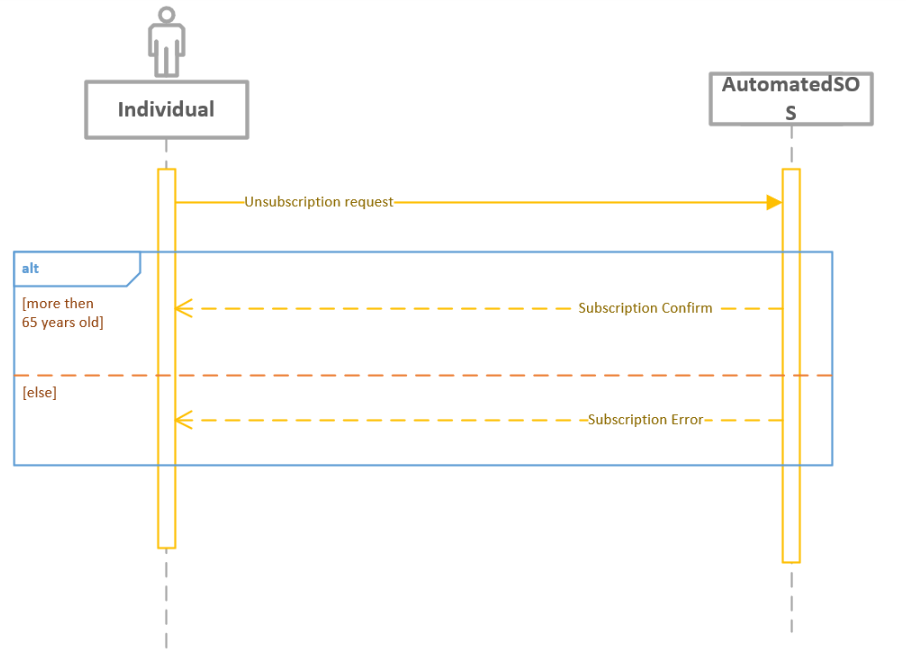
\includegraphics[scale=0.68]{pictures/ASOSubscriptionRequest.png}}
                \caption{Sequence diagram representing the subscription request for ASOS service.}
                \label{fig:ASOS-seq-diagram1}
            \end{figure}
            
        \subsubsection{Ambulance dispatching}
                Whenever the system receives a value that goes beyond the critical threshold, ASOS contacts the ambulance service, asking for assistance.
                
            \begin{table}[H]
            	\centering
                
                \begin{tabular}{|p{3cm}|p{8.2cm}|}
                    \hline
                    \textbf{Actors} & \begin{itemize}
                        \item Elderly person
                        \item Ambulance service
                    \end{itemize} \\
                     \hline
                    \textbf{Entry Condition} & The user has an ASOS account and is logged in. \\
                     \hline
                    \textbf{Events Flow} & \begin{enumerate}
                                               \item D4H collects through the connected device the Elderly person's data.
                                               \item ASOS checks if the values are beyond the critical threshold.
                                               \item If so, ASOS contacts the ambulance service, giving the location of the Elderly person gathered with the last measurement. Otherwise, it does nothing.
                                               \item The ambulance service sends an ambulance to the Elderly person location.
                                           \end{enumerate} \\
                     \hline
                    \textbf{Exit Condition} & The ambulance service has been warned and an ambulance in arriving at the Elderly person place. \\
                     \hline
                    \textbf{Exception} & There are no exceptions. \\
                     \hline
                \end{tabular}  
            \end{table}                 
            
            \begin{figure}[H]
                \centering
                \makebox[\textwidth][c]{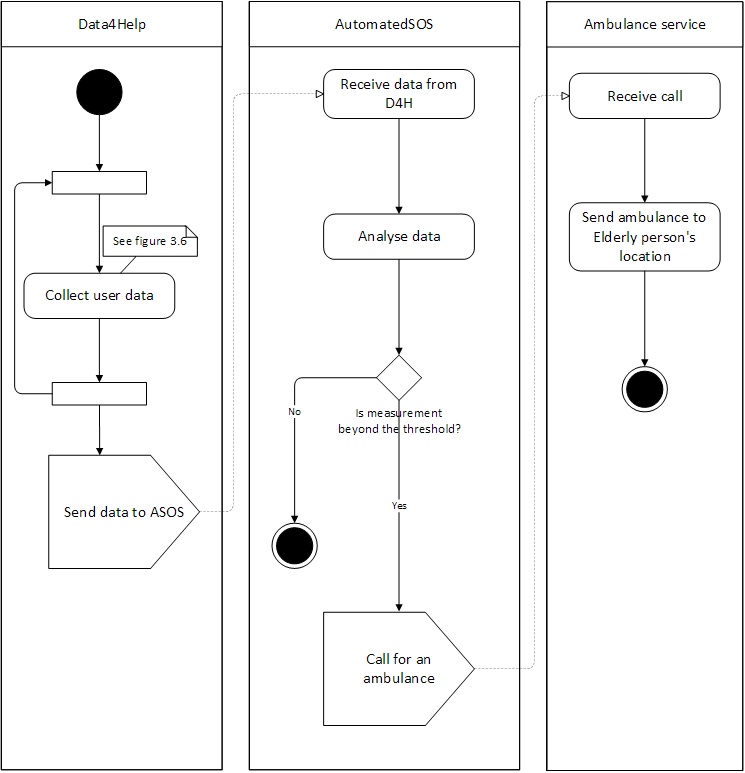
\includegraphics[scale=0.6150]{pictures/Activity1.png}}
                \caption{Activity diagram representing the call for an ambulance that ASOS performs when a critical measurement is collected by D4H. See figure \ref{fig:Data-storage-activity-diagram} to see how D4H collects user data.}
                \label{fig:ASOS-activity-diagram1}
            \end{figure}
            
    \subsection{Track4Run}
        Consider the following scenario:
        
        RunTogether is a group interested in the organisation of runs in Milan. After \emph{TrackMe} has launched \emph{Track4Run}, the company decides to download \emph{Track4Run} Organiser edition and to register to the service. It then tries to publish a run held at Parco Sempione, on 11/11/2018 at 9.30, allowing 30 participants. Since there is another run scheduled at the same place and time, \emph{Track4Run} shows an error message. RunTogether then decides to delay the competition until 12 and manages to publish it successfully. It then receives a confirmation mail with the summary of the process.
        
        Matteo enjoys jogging and wants to try to compete in a race. Therefore, he downloads \emph{Data4Help} application on his smart-phone and registers to the service. Then, he downloads \emph{Track4Run} application and searches for the runs available in Milan in November. He then selects RunTogether's race, since it still has open slots, and enrols in it, pressing on the specific button. \emph{Track4Run} sends him an email as confirmation.
        Fifteen minutes before the beginning of the race, Matteo is asked, through his D4H account, if he allows the acquisition of data, requested by T4R in order to track him during the race. He accepts.
        
        The day of the race, Matteo's girlfriend, Jessica, wants to follow his route during the run. Therefore, she downloads \emph{Track4Run}, without needing to register. She finds the run Matteo is enrolled in and selects it. \emph{Track4Run} then requests the map of the area from Google Maps and sends it back to Jessica with the location of the participants updating in real time. Since she followed the race until the end, the rank is shown to her.
        
        At the end of the race, Matteo wants to see the rank, so he opens \emph{Track4Run}, taps on the rank history tab and finally selects the run he just attended. The system promptly shows the result to him.
        
        \begin{figure}[H]
            \centering
            \makebox[\textwidth][c]{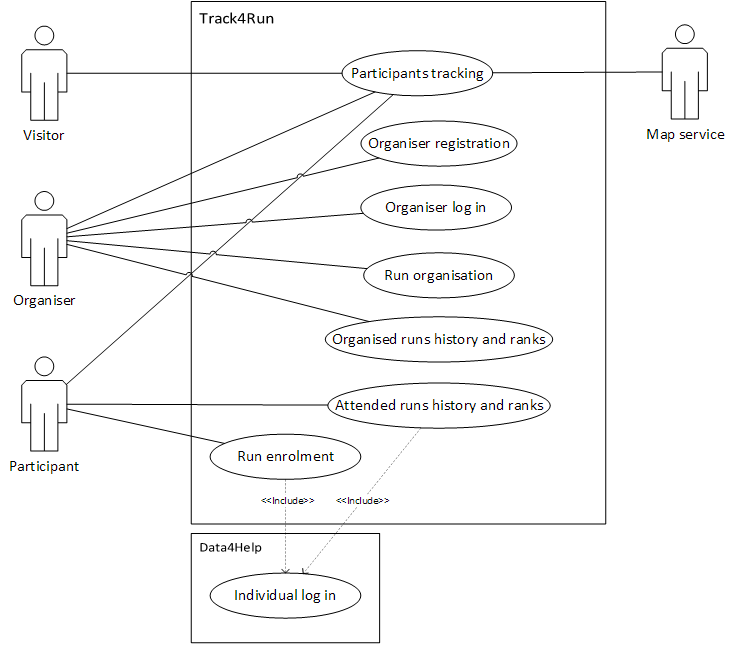
\includegraphics[scale=0.64]{pictures/T4R_UseCaseDiagram.png}}
            \caption{Use case diagram relative to \emph{Track4Run}. You can see the full use case diagram of D4H in the figure \ref{fig:D4H-Use-case-diagram}.}
            \label{fig:T4R-Use-case-diagram}
        \end{figure}        
        
        \subsubsection{Organiser registration and log in}
            Any Organiser needs to register to T4R before being able to organise and publish races. This account is in no way dependant to D4H and Organisers do not need to be registered to D4H too. Therefore, if they are already registered to D4H as Third-parties, they still need a new account, but can use the same information provided for D4H. 
            
            \begin{table}[H]
            	\centering
                
                \begin{tabular}{|p{3cm}|p{8.2cm}|}
                    \hline
                    \textbf{Actors} & \begin{itemize}
                        \item Visitor
                        \item Organiser
                    \end{itemize} \\
                     \hline
                    \textbf{Entry Condition} & There is no entry condition. \\
                     \hline
                    \textbf{Events Flow} & \begin{enumerate}
                                               \item The Visitor accesses the application log in page.
                                               \item The Visitor clicks on the ``\emph{Sing up now}" link and then fills in all the mandatory information (company name, VAT code, email and password).
                                               \item T4R creates a new account and sends a confirmation email to the just registered Organiser.
                                               \item The newly registered Organiser can now log into the application using the email and password previously provided, so to have access to the available features.
                                           \end{enumerate} \\
                     \hline
                    \textbf{Exit Condition} & The Organiser is registered and able to log into \emph{Track4Run}. \\
                     \hline
                    \textbf{Exception} & The Visitor is not able to register because the email or the VAT code are already in use. \newline
                                         A registered Organiser is not able to log in because the email or password inserted are wrong or the email has not been confirmed. \newline
                                         These exception will be handled by the system sending an error message. \\
                                         \hline
                \end{tabular}  
            \end{table}
            
            \begin{figure}[H]
                \centering
                \makebox[\textwidth][c]{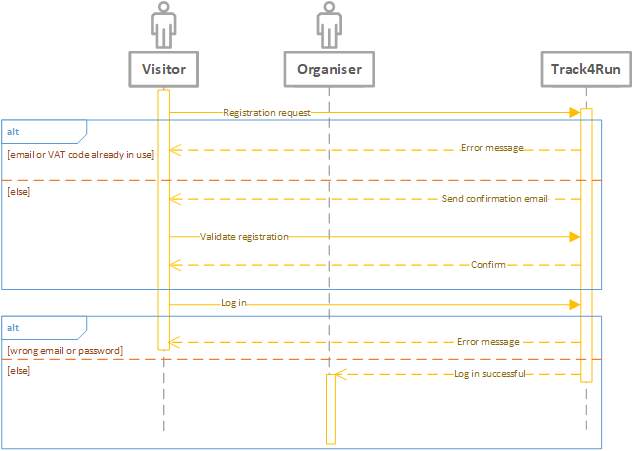
\includegraphics[scale=0.73]{pictures/Sequence4.png}}
                \caption{Sequence diagram representing the registration of an Organiser to T4R.}
                \label{fig:Organiser-registration-sequence-diagram}
            \end{figure}
            
        \subsubsection{Run organisation}
            
            The T4R system allows registered organisers to organise a run. They have to specify the time and the place, but it is not possible to add if there is another, already stored, race in the same place and at the same time. Different runs at the same time but different place are allowed.
            
            \begin{table}[H]
            	\centering
                
                \begin{tabular}{|p{3cm}|p{8.2cm}|}
                    \hline
                    \textbf{Actors} & \begin{itemize}
                        \item Organiser
                    \end{itemize} \\
                     \hline
                    \textbf{Entry Condition} & Organiser must have an organiser account in T4R system.\\
                     \hline
                    \textbf{Events Flow} & \begin{enumerate}
                                        \item The Organiser presses on ``\emph{New Run}" button.
                                        \item The Organiser specifies date, time, place and the maximum number of participants.
                                        \item The Organiser clicks on the ``\emph{Path}" button.
                                        \item T4R checks if there are no other races in the same place at the same time.
                                        \item If there are not, T4R asks Google Maps to provide the map of the location to the Organiser.
                                        \item Google Maps sends the map of the location to the Organiser.
                                        \item The Organiser keeps selecting the positions that define the path he wants to create until he is satisfied.
                                        \item Google Maps sends the finalised path to T4R.
                                        \item T4R sends to the Organiser a confirmation email.
                                            \end{enumerate}\\
                     \hline
                    \textbf{Exit Condition} & A new race has been created.\\
                     \hline
                    \textbf{Exception} & If there is another stored race with the same data, time and location, the system                       handles the exception, showing an error message to the organiser. \\
                     \hline
                \end{tabular}  
            \end{table} 
            
            \begin{figure}[H]
                \centering
                \makebox[\textwidth][c]{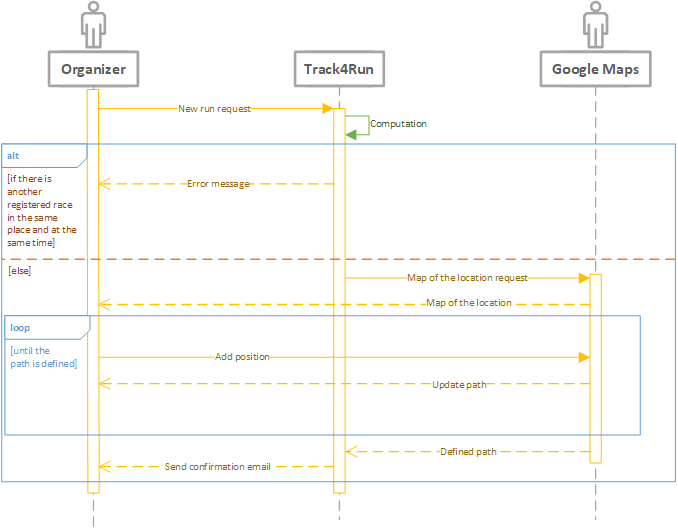
\includegraphics[scale=0.71]{pictures/RunOrganizationSequenceDiagram.png}}
                \caption{Sequence diagram representing the request performed to create a new run.}
                \label{fig:T4R-run-organization}
            \end{figure}
            
        \subsubsection{Enrolment to a run}
            Any Participant can log into T4H using his D4H (Individual) account. After doing that, he/she will be able to see all available runs and to enrol to them. The races can be filtered by time and zone, as to simplify the research.
            
            \begin{table}[H]
            	\centering
                
                \begin{tabular}{|p{3cm}|p{8.2cm}|}
                    \hline
                    \textbf{Actors} & \begin{itemize}
                        \item Participant
                    \end{itemize} \\
                     \hline
                    \textbf{Entry Condition} & The Participant is logged into T4R, using his D4H Individual account. \\
                     \hline
                    \textbf{Events Flow} & \begin{enumerate}
                                                \item The participant clicks on the ``\emph{enroll run}" button.
                                                \item The Participant looks through the available races, eventually filtering them to ease the search, and selects one of them.
                                                \item The Participant presses on ``\emph{Enrol}" button.
                                                \item T4R sends a confirmation mail to the Participant.
                                            \end{enumerate}\\
                     \hline
                    \textbf{Exit Condition} & The Participant is enrolled to the selected race.\\
                     \hline
                    \textbf{Exception} & If the Participant is already enrolled to another race at the same time, an                          error message is sent to him/her. \newline
                                         If the race has reached the maximum number of subscriptions, an error message is sent to the Participant. \\
                     \hline
                \end{tabular}  
            \end{table}            
            
            \begin{figure}[H]
                \centering
                \makebox[\textwidth][c]{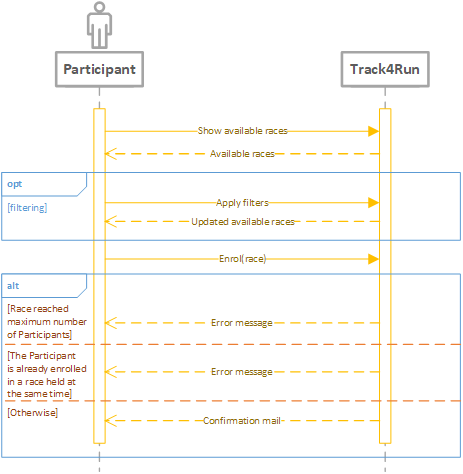
\includegraphics[scale=0.97]{pictures/modelT4R_ParticipantEnrollment.png}}
                \caption{Sequence diagram representing the enrolment to a run of a Participant.}
                \label{fig:T4R-participant-enrolment}
            \end{figure}
            
        \subsubsection{Participant tracking}
            
            Every Visitor, registered or not, is able to track participants on a map during the race and, if there is more then one run at the same time, they can choose which run to watch. To provide this service, the system interacts with Google Maps. This can be done in both the Organisers edition and normal T4R application.
            In order to ask the permission to track the runners, T4R performs a single user data request with subscription through D4H for each of them. Therefore, in order to effectively participate to the run, each Participant has to accept the request, otherwise he gets removed from the race. The way the request is performed is shown in figure \ref{fig:IndividualRequest}, where T4R acts as a Third-party.
            
            \begin{table}[H]
            	\centering
                
                \begin{tabular}{|p{3cm}|p{8.2cm}|}
                    \hline
                    \textbf{Actors} & \begin{itemize}
                                            \item User
                                            \item Map service
                                        \end{itemize} \\
                     \hline
                    \textbf{Entry Condition} & T4R have to do an "Individual request" to D4H for each ranners. \\
                     \hline
                    \textbf{Events Flow} & \begin{enumerate}
                                                \item The User launches the application.
                                                \item They press on the ``\emph{Track runners}" button.
                                                \item The system shows the list of current runs.
                                                \item The User selects the run of interest.
                                                \item D4H sends computed position to T4R.
                                                
                        \item T4R sends to Map service runners position
                                                \item The map service sends to T4R map and runners location.
                                                \item The system shows the map with all runners current position.
                                                \item If the User follows the run until the end, T4R shows to him the rank.
                                            \end{enumerate} \\
                     \hline
                    \textbf{Exit Condition} & Users are now able to see runners on a map (and the rank if the stay until the race is over). \\
                     \hline
                    \textbf{Exception} & 
                    \begin{itemize}
                        \item If there are no runs in that moment, the system handles the exception, showing a notification message.
                        \item If the user disconnects, the system doesn't show Participant tracking anymore.
                    \end{itemize} \\
                     \hline
                \end{tabular}  
            \end{table}
            
            \begin{figure}[H]
                \centering
                \makebox[\textwidth][c]{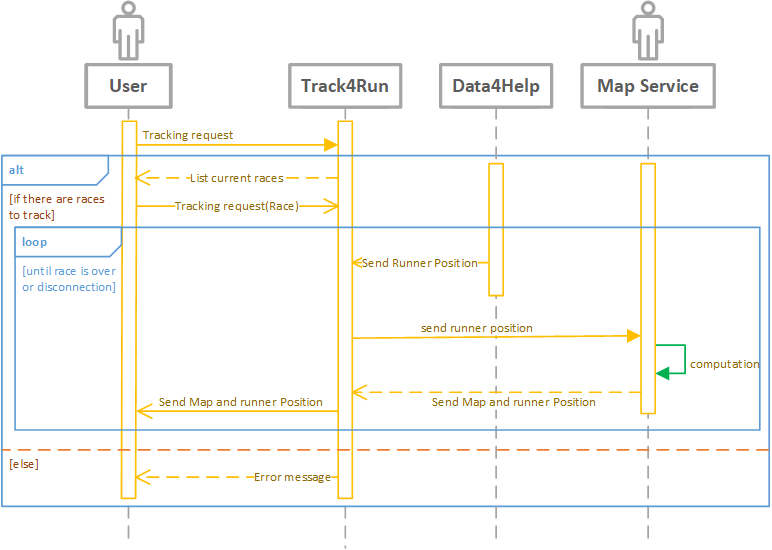
\includegraphics[scale=0.80]{pictures/participantTrackingSequenceDiagram.png}}
                \caption{Sequence diagram representing the request in order to see participant position on a map during the run.}
                \label{fig:T4R-runner-tracking}
            \end{figure}
            
        \subsubsection{Rank history}
            Participants and Organisers are able to see the rank for all past races they have took part in or organised, respectively. Since the procedure to access the rank history is the same for the two actors, only one use case is provided. Of course, the two actors use the versione of the application dedicated to them.

            \begin{table}[H]
            	\centering
                
                \begin{tabular}{|p{3cm}|p{8.2cm}|}
                    \hline
                    \textbf{Actors} & \begin{itemize}
                                            \item Participant / Organiser
                                        \end{itemize} \\
                     \hline
                    \textbf{Entry Condition} & The Participant has took part in / The Organiser has organised at least                              one run and is logged in. \\
                     \hline
                    \textbf{Events Flow} & \begin{enumerate}
                                                \item The Participant / Organiser clicks on the ``\emph{Ranking}" tab.
                                                \item T4R shows the rank to the Participant / Organiser.
                                            \end{enumerate} \\
                     \hline
                    \textbf{Exit Condition} & The Participant / Organiser is able to see the rank of the selected race                             he/she has took part in / organised. \\
                     \hline
                    \textbf{Exception} & If the Participant has not took part in any run, an error                       message is sent to him/her. \newline
                                         If the Organiser has not organised any run, an error message is sent to him/her. \\
                     \hline
                \end{tabular}  
            \end{table}
            
            \begin{figure}[H]
                \centering
                \makebox[\textwidth][c]{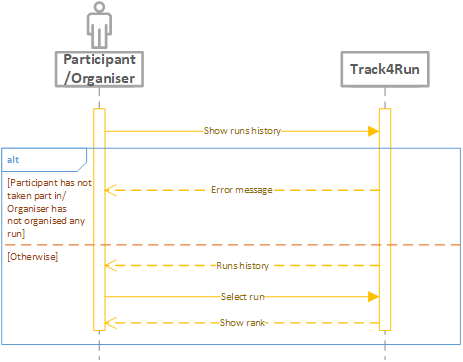
\includegraphics[scale=0.97]{pictures/modelT4R_RankHistory.png}}
                \caption{Sequence diagram representing request for the rank of a run.}
                \label{fig:T4R-rank-history}
            \end{figure}
            
    \subsection{Traceability matrix}
    
    In this section, we will keep track of the relationship between goals, requirements and use cases. In order to do this, we build for each analysed service \emph{Traceability matrix}. It is important to highlight that the same use case could be linked to different requirements and the same requirement to different use cases. 
    
        \subsubsection{Data4Help}
            \definecolor{light}{HTML}{FFF9C4}
            \definecolor{dark}{HTML}{FFF59D}
        
         \begin{table}[H]
            	\centering
                \rowcolors{2}{dark}{light}
                \begin{tabular}{|c|c|c|}
                    \hline
                    \rowcolor[HTML]{FDD835} \textbf{ GOAL} & \textbf{ REQUIREMENT} & \textbf{USE CASE ID}\\
                    \hline
                    \ref{goal1 : monitoring} & \ref{R1-Individual-registration} & Individual registration/log \\
                    \hline
                     \ref{goal1 : monitoring} & \ref{R1-third-party-registration} & Third-party registration and log in\\
                    \hline
                    \ref{goal1 : individual monitoring} & \ref{R1-individual-request} & Single user data request and subscription\\
                    \hline
                    \ref{goal1 : subscription} & \ref{R1-third-party-subscription} & Single user data request and subscription\\
                    \hline
                    \ref{goal1: individual privacy} & \ref{R1-individual-accept-request} & Single user data request and subscription\\
                    \hline
                    \ref{goal1: individual privacy} & \ref{R1-individual-refused-request} & Single user data request and subscription\\
                    \hline
                    \ref{goal1 : subscription}  & \ref{R1-unsubscription} & Single User data unsubscription\\
                    \hline
                    \ref{goal1 : subscription} & \ref{R1-Individual-unsubscription} & Single User data unsubscription\\
                    \hline
                    \ref{goal1 : subscription} & \ref{R1-third-party-subscription}& Aggregated user data request and subscription\\
                    \hline
                    \ref{goal1 : group monitoring} & \ref{R1-group-requests}& Aggregated user data request and subscription\\
                    \hline
                    \ref{goal1 : group monitoring} & \ref{R1-group-req-approuved}& Aggregated user data request and subscription\\
                    \ref{goal1 : group monitoring} & \ref{R1-group-request-refused}& Aggregated user data request and subscription\\
                    \hline
                    \ref{goal1 : group monitoring} & \ref{R1-group-data-anonymized}& Aggregated user data request and subscription\\
                    \hline
                    \ref{goal1 : subscription} & \ref{R1-unsubscription}& Aggregated user data unsubscription\\
                    \hline
                    \ref{goal1 : subscription} & \ref{R1-third-party-unsubscription}& Aggregated user data unsubscription\\
                    \hline
                    \ref{goal1 : subscription} & \ref{R1-subscription-updates} & Collected data during Subscription \\
                     \hline
                    \ref{goal1: individual privacy} &\ref{R1-gathered-data}  & Data Collection and Visualisation\\
                     \hline
                    \ref{goal1: individual privacy} &\ref{R1-individual-personal-data}  & Data Collection and Visualisation\\
                    \hline
                    \ref{goal1 : monitoring} & \ref{R1-history-request}& Third-parties request history \\
                    \hline
                \end{tabular}  
            \end{table}
        
        
        \subsubsection{AutomatedSOS}
            \definecolor{light}{HTML}{B3E5FC}
            \definecolor{dark}{HTML}{81D4FA}
        
        \begin{table}[H]
            	\centering
                \rowcolors{2}{dark}{light}
                \begin{tabular}{|c|c|c|}
                    \hline
                    \rowcolor[HTML]{03A9F4} \textbf{ GOAL} & \textbf{ REQUIREMENT} & \textbf{USE CASE ID}\\
                    \hline
                    \ref{goal2 : status monitorin} & \ref{R2-subscription}& Subscription Request\\
                    \hline
                    \ref{goal2 : ambulance}  & \ref{R2-data-and-ambulance} & Ambulance dispatching\\
                    \hline
                \end{tabular}  
            \end{table}

        \subsubsection{Track4Run}
            \definecolor{light}{HTML}{DCEDC8}
            \definecolor{dark}{HTML}{C5E1A5}
        
        \begin{table}[H]
            	\centering
                \rowcolors{2}{dark}{light}
                \begin{tabular}{|c|c|c|}
                    \hline
                     \rowcolor[HTML]{8BC34A} \textbf{ GOAL} & \textbf{ REQUIREMENT} & \textbf{USE CASE ID}\\
                    \hline
                    \ref{goal3 : run organization} & \ref{R3-organizer-registration} & Organiser registration and log in\\
                    \hline
                    \ref{goal3 : run organization}  & \ref{R3-run-organization} & Run organisation\\
                    \hline
                    \ref{goal3 : run organization}  & \ref{R3-run-different-time} & Run organisation\\
                    \hline
                    \ref{goal3 : enrolling}  & \ref{R3-login-enrollin} & Enrolment to a run\\
                    \hline
                    \ref{goal3 : enrolling}  & \ref{R3-enrolling-different-time}& Enrolment to a run\\
                    \hline
                    \ref{goal3 : enrolling}  & \ref{R3-decreasing-participant-number}& Enrolment to a run\\
                    \hline
                    \ref{goal3 : tracking}  & \ref{R3-visitors} & Participant tracking\\
                    \hline
                     \ref{goal3 : tracking}  & \ref{R3-ranking-end} & Participant tracking\\
                    \hline
                     \ref{goal3 : run organization} \ref{goal3 : enrolling}  & \ref{R3-ranking-storage}& Rank history\\
                    \hline
                \end{tabular}  
            \end{table}